% You can submit either a single PDF file that includes the manuscript text
% and any display items, or separate files for text, figures and tables.
%
% 1500 words, excluding the introductory paragraph, online Methods,
% references and figure legends
%
% TODOs
% - cover letter
% - names and affiliations of all co-authors; current addresses
% - Author contributions
% - Acknowledgements
%
% - references: Gregg Neuron

\documentclass[letterpaper]{article}
%\documentclass[12pt,letterpaper]{article}
%\setlength{\textwidth}{480pt}
%\setlength{\textheight}{630pt}
%\setlength{\voffset}{0pt}

\usepackage{amsmath, geometry, graphicx, tikz}
\usepackage{float}
\usetikzlibrary{arrows.meta}
\bibliographystyle{plain}

% https://tex.stackexchange.com/questions/6758/how-can-i-create-a-bibliography-like-a-section
\usepackage{etoolbox}
\patchcmd{\thebibliography}{\section*}{\section}{}{}

\pagestyle{plain}

%\title{Variation of Genomic Imprinting in the Human Brain}
\title{Unperturbed Expression Bias of Imprinted Genes in Schizophrenics}
\author{Attila Guly\'{a}s-Kov\'{a}cs\(^\ddagger\), Ifat Keydar\(^\ddagger\),
...,
%\\
%Eva Xia, Menachem Fromer, Doug Ruderfer,\\
%Ravi Sachinanandam,
Andrew Chess\(^\ast\)}

\date{Icahn School of Medicine at Mount Sinai}

\begin{document}

\maketitle
\begin{center}
\(\ddagger\) equal contribution;
\(\ast\) correspondence: andrew.chess@mssm.edu
\end{center}

%\clearpage
\tableofcontents

\clearpage

\section{Main text}

How inter-individual differences in gene regulation correlates with disease is
beginning to be examined through analyses of RNA-seq from post-mortem brains
of individuals with schizophrenia and from control brains~\cite{Fromer2016a}.
Here we focus on differences in allele-specific expression, following up on
the CommonMind Consortium (CMC http://www.synapse.org/CMC) RNA-seq analyses of
\(>500\) human dorsolateral prefrontal cortex (DLPFC) samples.  We find that the
fraction of imprinted human genes is consistent with lower (\(\approx 0.5
\%\))~\cite{Perez2015,DeVeale2012,Baran2015} as opposed to
higher~\cite{Gregg2010a} estimates in mice. The handful of novel potentially
imprinted genes we find are all in close genomic proximity to known imprinted
genes.  Analyzing the extent of allelic expression bias---a hallmark of
imprinting---across hundreds of individuals allowed us to examine its
dependence on various factors.  We find that allelic bias is independent of
the diagnosis of schizophrenia.  In contrast
age up or down-regulates allelic bias of some imprinted genes and genetic
ancestry also has an impact.

The observation~\cite{Noor2015,Rees2014} that maternally derived
microduplications at 15q11-q13---harboring the imprinted gene UBE3A---may not
only cause Prader-Willi syndrome, but are also highly penetrant for
schizophrenia has raised the possibility that perturbation of regulation of
imprinted genes in general may play a role in psychotic disorders.  As it is
known that the extent of imprinting of individual genes varies over different
tissues we chose the DLPFC region, which controls complex cognitive and
executive functions and is known to display functional abnormalities in
schizophrenia.  We obtained pre-publication DLPFC RNA-seq data from the CMC
and analyzed allele-specific expression with the idea of (i) identifying
imprinted genes in the adult human brain and (ii) explaining the
variability in allelic bias across 579 individuals in terms of their
psychiatric diagnosis, age at death, etc.  This was facilitated by the
balanced case-control groups (258 SCZ, 267 Control, 54 bipolar or other
affective/mood disorder, AFF) and the large age variability.

For each individual \(i\) and gene \(g\) we quantified allelic bias based on
RNA-seq reads using a statistic called \emph{read count ratio} \(S_{ig}\)
(Fig.~\ref{fig:study-design}, Methods), which ranges from 0.5 to 1 indicating unbiased
biallelic expression (at 0.5), some allelic bias (at intermediate values) or
strictly monoallelic expression (at 1).  We corrected for a number
of factors this approach is known to be sensitive to.  We quality-filtered
RNA-seq reads and helped distinguish allele-specific reads using DNA
genotyping data before calculating \(S\) and then applied post hoc corrections
for mapping bias (Methods).

A total of \(5307\) genes passed our filters designed to remove genes with
scarce RNA-seq data reflecting low expression and/or low coverage of RNA-seq.
Fig.~\ref{fig:ranking-genes} presents the conditional empirical distribution
of \(S_{\cdot g}\) across all individuals given each gene \(g\).  The observed wide
\(S_{\cdot g}\) distributions suggest large across-individuals variation of allelic bias for all
genes, even if a substantial component of the \(S_{\cdot g}\) variation originates from technical sources.
Still, as expected, for many genes known to be imprinted in mice or in other human tissues
(referred to as \emph{known imprinted} genes like PEG10, ZNF331) the distribution of \(S_{\cdot g}\) was shifted
to the right signaling strong allelic bias (Fig.~\ref{fig:ranking-genes}, upper
half).

To identify imprinted genes in the human adult DLPFC we defined the score of
each gene \(g\) as the fraction of individuals \(i\) for whom \(S_{ig}>0.9\).
We ranked all 5307 genes according to their score
(Fig.~\ref{fig:ranking-genes} bottom right).  The heat map of the \(S_{\cdot
g}\) distribution for ranked genes (Fig.~\ref{fig:ranking-genes}, lower left)
shows that the top \(50\) genes, which constitute \(\approx 1\%\) of all genes
in our analysis, are qualitatively different from the bottom \(\approx 99\%\)
exhibiting strongly right-shifted distribution of \(S_{\cdot g}\)
characteristic to imprinting.

29 of the top-scoring 50 genes fell into previously described imprinted gene
clusters (Fig.~\ref{fig:clusters}); 21 of these 29 are \emph{known imprinted}
genes and 8 are \emph{nearby candidates} (blue and green bars in
Fig.~\ref{fig:top-genes}).   \emph{A priori} the expectation is that
\emph{known imprinted} genes \emph{nearby candidates} are much more likely to
be imprinted  in the present data set than \emph{distant candidates} (the
genes outside clusters, Fig.~\ref{fig:top-genes}, red bars).  We combined this
prior expectation with two tests based on our data to distinguish imprinting
from alternative causes of high read count ratio such as mapping bias and
cis-eQTL effects (see Methods: Reference/non-reference allele test and Test
for nearly unbiased allelic expression).  The results of both tests (X's and
black bars, Fig.~\ref{fig:top-genes}) agreed well with the \emph{a priori}
expected status.  This prompted us to call imprinted in the adult human DLPFC
all \emph{known imprinted} and \emph{nearby candidate} genes within the top
50.  We included also the \emph{known imprinted} gene UBE3A, which ranked
below 50 but whose score was still substantial (Fig.~\ref{fig:known-genes})
yielding 30 imprinted genes (panel headers in
Fig.~\ref{fig:S-Dx}-\ref{fig:S-age}).

Getting at the central question of our work Fig.~\ref{fig:S-Dx} shows
that read count ratio is similarly distributed in the Control, SCZ and AFF
group for all 30 imprinted genes suggesting independence between allelic bias and diagnosis of
schizophrenia.

To confirm this rigorously we performed statistical inference using mixed
effects models (Methods), which can capture much of the complex pattern of
dependencies in genomic data including those we observed within and between
technical and biological explanatory variables (Table~\ref{tab:predictors},
Fig.~\ref{fig:predictor-associations}), and which gain power from letting
genes ``borrow strength from each other'' (Fig.~\ref{fig:glm-vs-hierarch}).
We fitted many alternative mixed models, selected the best-fitting one using
the Akaike Information Criterion (AIC) and confirmed the goodness of fit with
diagnostic plots (Methods,
Fig.~\ref{fig:qqnorm-mixed},~\ref{fig:homoscedas-mixed}).

Based on the best fitting model (henceforth ``the model'') we could formally
reject the hypotheses that read count ratio depends on diagnosis as either
main effect or interaction (see term \((1\mid\mathrm{Dx})\) and
\((1\,|\,\mathrm{Dx}:\mathrm{Gene})\) in Table~\ref{tab:mod-sel},
respectively).  That this key result is not due to low power is indicated by
the highly significant dependence of read count ratio on gene identity
(see \((1\mid\mathrm{Gene})\) in Table~\ref{tab:mod-sel} and compare panels in
Fig.~\ref{fig:S-Dx}).

Fig.~\ref{fig:S-age} suggests that the read count ratio depends negatively on
age for some imprinted genes, depends positively for others, and is
independent of age for the rest of imprinted genes.  This apparent
dependence might be indirect, i.e.~one that is mediated by some variable(s)
``inbetween'' age and read count ratio
(Fig.~\ref{fig:predictor-associations},~\ref{fig:glm-vs-hierarch}) but
the model allowed us to isolate the direct component of age dependence: we
found that the gene-specific random age effect is indeed significant even if
no fixed effect---which would be shared by all imprinted genes---was supported
(see \((\mathrm{Age}\,|\,\mathrm{Gene})\) and \(\mathrm{Age}\), respectively,
in Table~\ref{tab:mod-sel}).

Based on the model we also predicted
gene-specific regression coefficients mediating the direct component of age
effect (Fig.~\ref{fig:pred-rnd-coefs} top middle).  The predicted coefficients
agreed well with all but a few panels of Fig.~\ref{fig:S-age} the latter of
which (e.g.~UBE3A) therefore represent purely indirect dependence.

The same type of analysis on the effects of ancestry principal components and
gender gave similar results: while the fixed effect, shared by all genes, of
these variables was negligible, three of the random, gene-specific, effects
received significant support.  These three, ordered by decreasing
statistical significance, are
\((\mathrm{Ancestry.1}\,|\,\mathrm{Gene})\),
\((\mathrm{Ancestry.3}\,|\,\mathrm{Gene})\) and
\((1\,|\,\mathrm{Gender}:\mathrm{Gene})\) (Table~\ref{tab:mod-sel}).  The
corresponding predicted random coefficients are presented in
Fig.~\ref{fig:pred-rnd-coefs}.

In summary age, ancestry, and to a lesser extent gender, are suggested by our
model-based analysis to exert effect on allelic bias in a way that the
direction and magnitude of the effect varies across genes.

The number of imprinted genes in the mammalian brain has been controversial:
some early genome wide studies~\cite{Gregg2010a,Gregg2010} estimated over a
thousand, suggesting that the number of imprinted genes in the brain is an
order of magnitude greater than in other tissues.  Later work cast doubt on
the methodology used and found that the number of imprinted genes in brain is
in line with expectations from studies of other tissues, identifying only a
handful of new candidate imprinted genes in brain
~\cite{Perez2015,DeVeale2012,Baran2015}.  Based on 579 postmortem human DLPFC
samples we find evidence supporting only a handful of novel imprinted genes
all of which reside in genomic locations nearby to known imprinted genes.
Thus our results support those more recent studies that found no large excess
of imprinted genes in the brain.

The large size of our sample and the case-control makeup allowed us to explore
the potential for correlation of extent of imprinting in the DLPFC with
schizophrenia.  Although our approach gave strong support for dependence of
imprinting on age and ancestry, no dependence on schizophrenia was detected
either when we assumed that the dependence is the same for all imprinted genes
or that it varies across genes.  Thus our data indicate that imprinting in the
DLFPC does not play a significant role in schizophrenia in contradiction of
the ``imprinted brain'' hypothesis~\cite{Crespi2008}.  Given the complex
genetic architecture of schizophrenia~\cite{Sullivan2012} as well as technical
noise in postmortem brain RNA studies there could still be some correlation of
the extent of imprinting and schizophrenia.

We found that imprinting depends on ancestry in a gene
specific manner but the type of dependence that is shared by all imprinted
genes was not supported.  This is expected because the studied
ancestry variables must incorporate some of the cis expression
QTLs in imprinted genes such that those eQTLS perturb allelic bias in a gene
specific manner.

Our finding that imprinting depends on age in later adulthood is rather
intriguing.  Age dependence through early postnatal life supported
experimentally~\cite{Perez2015} but such dependence during later adulthood has
so far only been predicted~\cite{Ubeda2012} based on a hypothesis that links
``genomic imprinting and the social brain''~\cite{Isles2006}.  Previous
genomics studies~\cite{Baran2015} were statistically underpowered to address
this question in humans.  Although our age-related finding supports the
``social brain'' hypothesis, it leaves the possibility open that the observed
age related changes indicate merely the loss of tight regulation of those
genes with aging.


\clearpage

\section{Methods}

\subsection{Defining the read count ratio to quantify allelic bias}

We quantified allelic bias based on RNA-seq reads using a statistic called
\emph{read count ratio} \(S\), whose definition we
based on the total read count \(T\) and the \emph{higher read count} \(H\),
i.e.~the count of reads carrying only either the reference or the alternative SNP variant,
whichever is higher.  The
definition is
\begin{equation}
S_{ig} = \frac{H_{ig}}{T_{ig}}= \frac{\sum_s H_s}{\sum_sT_s},
\label{eq:S-definition}
\end{equation}
where \(i\) identifies an individual, \(g\) a gene, and the summation runs
over all SNPs \(s\) for which gene \(g\) is heterozygous in individual \(i\) (Fig.~\ref{fig:study-design}).
Note that if \(B_{ig}\) is the count or reads that map to the \(b_{ig}\) allele
(defined as above) and if we make the same distributional assumption as above, namely that \(B_{ig}\sim
\mathrm{Binom}(p_{ig}, T_{ig})\), then \(\mathrm{Pr}(H_{ig}=B_{ig}|p_{ig})\), the probability of correctly
assigning the reads with the higher count to the allele towards which
expression is biased, tends to 1 as \(p_{ig} \rightarrow 1\).  We took
advantage of this theoretical result in that we subjected only those genes to
statistical inference, whose read count ratio was found to be high and,
therefore, whose \(p_{ig}\) is expected to be high as well.

Fig.~\ref{fig:study-design} illustrates the calculation of \(S_{ig}\) for the
combination of two hypothetical genes, \(g_1,g_2\), and two individuals,
\(i_1,i_2\).  It also shows an example for the less likely event that the lower rather
than the higher read count corresponds to the SNP variant tagging the higher
expressed allele (see SNP \(s_3\) in gene \(g_1\) in individual \(i_2\)).

Before we carried out our read count ratio-based analyses, however, we cleaned
our RNA-seq data by quality-filtering and by improving the accuracy of SNP
calling with the use of DNA SNP array data and imputation. In the following
subsections of Methods we describe the data, these procedures, as well as our
regression models in detail.

\subsection{Brain samples, RNA-seq}

Human RNA samples were collected from the dorsolateral prefrontal cortex of
the CommonMind consortium from a total of \(579\) individuals after
quality control. Subjects included 267 control individuals, as well as 258
with schizophrenia (SCZ) and 54 with affective spectrum disorder (AFF).
RNA-seq library preparation uses Ribo-Zero (which selects against ribosomal
RNA) to prepare the RNA, followed by Illumina paired end library generation.
RNA-seq was performed on Illumina HiSeq 2000.

\subsection{Mapping, SNP calling and filtering}

We mapped 100bp, paired-end RNA-seq reads (\(\approx50\) million reads per sample) using Tophat
to Ensembl gene transcripts of the human genome (hg19; February, 2009) with
default parameters and 6 mismatches allowed per pair (200 bp total). We
required both reads in a pair to be successfully mapped and we removed reads
that mapped to \(>1\) genomic locus. Then, we removed PCR replicates using the
Samtools rmdup utility; around one third of the reads mapped (which is
expected, given the parameters we used and the known high repeat content of
the human genome). We used Cufflinks to determine gene expression of Ensembl
genes, using default parameters. Using the BCFtools utility of Samtools, we
called SNPs (SNVs only, no indels). Then, we invoked a quality filter
requiring a Phred score \(>20\) (corresponding to a probability for an
incorrect SNP call \(<0.01\)).

We annotated known SNPs using dbSNP (dbSNP 138, October 2013). Considering all
579 samples, we find 936,193 SNPs in total, 563,427 (60\%) of which are novel.
Further filtering of this SNP list removed the novel SNPs and removed SNPs
that either did not match the alleles reported in dbSNP or had more than 2
alleles in dbSNP. We also removed SNPs without at least 10 mapped reads in at
least one sample. Read depth was measured using the Samtools Pileup utility.
After these filters were applied, 364,509 SNPs remained in 22,254 genes. These
filters enabled use of data with low coverage.  For the 579
samples there were 203 million reads overlapping one of the
364,509 SNPs defined above.  Of those 158 million (78\%) had genotype data
available from either SNP array or imputation.

\subsection{Genotyping and calibration of imputed SNPs}

DNA samples were genotyped using the Illumina Infinium SNP array. We used
PLINK with default parameters to impute genotypes for SNPs not present on the
Infinium SNP array using 1000 genomes data.  We calibrated the
imputation parameters to find a reasonable balance between the number of genes
assessable for allelic bias and the number false positive
calls since the latter can arise if a SNP is
incorrectly called heterozygous.

We first examined how many SNPs were heterozygous in DNA calls and had a
discordant RNA call (i.e.~homozygous SNP call from RNA-seq) using different imputation
parameters. Known imprinted genes were excluded. We examined RNA-seq reads
overlapping array-called heterozygous SNPs which we assigned a heterozygosity
score \(L_\mathrm{het}\) of 1, separately from RNA seq data
overlapping imputed heterozygous SNPs, where the \(L_\mathrm{het}\) score could
range from 0 to 1.  After testing different thresholds
we selected an \(L_\mathrm{het}\) cutoff of 0.95 (i.e. imputation confidence
level of 95\%), and a minimal coverage of 7 reads per SNP. With these
parameters, the discordance rate (monoallelic RNA genotype in the context of a
heterozygous DNA genotype) was 0.71\% for array-called SNPs and 3.2\% for
imputed SNPs.

The higher rate of discordance for the imputed SNPs
is due to imputation error.  These were taken into
account in two ways.
First, we considered all imputed SNPs for a gene \(g\) and individual \(i\)
jointly.  Second, we excluded
any individual, for which one or more SNPs supported biallelic
expression.

%At this point, the matrix includes 147
%million data points covering 213,208 SNPs, of which 114 million (77\%) have
%imputation data.

\subsection{Quality filtering}

\label{sec:filtering}

Two kind of data filters were applied sequentially: (1) a \emph{read
count-based} and (2) an \emph{individual-based}.  The read count-based filter
removes any such pair $(i,g)$ of individual $i$ and genes $g$ for which the
total read count $T_{ig}<t_\mathrm{rc}$, where the read count threshold
$t_\mathrm{rc}$ was set to 15. The individual-based filter removes any genes
$g$ (across all individuals) if read count data involving $g$ are available
for less than $t_\mathrm{ind}$ number of individuals, set to 25.
These final filtering procedures decreased the number of genes in the data from
\(15584\) to \(n=5307\).

\subsection{Reference/non-reference allele test to correct for mapping bias
and eQTLs}

We designed this test to distinguish imprinting from alternative causes of
high read count ratio (Fig.~\ref{fig:top-genes}): mapping bias or cis-eQTL
effects.  For any given gene this is a possibly compound test since there may
be multiple SNPs that are informative for the read count ratio (see Defining
the read count ratio above).

For a given gene the compound null hypothesis is that the observed high read
count ratio is due only to imprinting.  For each informative SNP this
hypothesis means that the reference and non-reference allele are associated
with equal probability to the \emph{higher read count} (see Methods: Defining
the read count ratio to quantify allelic bias).  Thus for each SNP we assumed
that the number of individuals for whom the reference allele is associated to
the \emph{higher read count} is binomially distributed with probability
parameter 0.5.  The we calculated the fraction of informative SNPs for which the
null hypothesis can be rejected at 0.05 significance level and used this
information to decide whether the compound null hypothesis for the gene itself
can be rejected.

\subsection{Test for nearly unbiased allelic expression}

The null hypothesis of this test is that the higher read count
\(H_{ig}=S_{ig}T_{ig}\) for gene \(g\) and individual \(i\) is drawn from a
binomial distribution with a probability parameter \(p_{ig}\approx 0.5\)
suggesting nearly unbiased allelic expression.  More specifically, the test
was defined by the criteria
\begin{equation}
S_{ig} \le 0.6 \text{ and } \mathrm{UCL}_{ig} \le 0.7,
\label{eq:unbiased-test}
\end{equation}
where the 95\% upper confidence limit \(\mathrm{UCL}_{ig}\) for the expected
read count ratio \(p_{ig}\) was calculated assuming that the higher read count
\(H_{ig}\sim \mathrm{Binom}(p_{ig}, T_{ig})\), on the fact that binomial
random variables are asymptotically (as \(T_{ig}\rightarrow \infty\)) normal
with \(\mathrm{var}(H_{ig}) = T_{ig}p_{ig}(1-p_{ig})\), and on the equalities
\(\mathrm{var}(S_{ig}) = \mathrm{var}(H_{ig}/T_{ig}) =
\mathrm{var}(H_{ig})/T_{ig}^2\).  Therefore
\begin{equation}
\mathrm{UCL}_{ig} = S_{ig} + z_{0.975} \sqrt{\frac{S_{ig} (1 - S_{ig})}{T_{ig}}},
\end{equation}
where $z_{p}$ is the $p$ quantile of the standard normal distribution.

\subsection{Mixed and fixed regression models}
\label{sec:methods-regression}

We modeled the dependence of read count ratio of imprinted genes on biological
and technical explanatory variables (Table~\ref{tab:predictors}) using mixed
and fixed generalized linear models (GLMs).

GLMs in general describe a conditional distribution of a response variable
\(y\) given a linear predictor \(\eta\) such that the distribution is from the
exponential family and that \(\mathrm{E}(y|\eta) = g^{-1} (\eta)\), where
\(g\) is some link function.  In the present context the response \(y\) is the
observed read count ratio that is possibly transformed to improve the model's
fit to the data.  We performed fitting with the lme4 and stats
R packages and tested several combinations of transformations, link
functions, and error distributions (Table~\ref{tab:model-names}).  For
inference we used the best fitting combination (\(\mathrm{unlm.Q}\),
Table~\ref{tab:model-names}) as assessed by the normality
(Fig.~\ref{fig:qqnorm-mixed}) and homoscedasticity
(Fig.~\ref{fig:homoscedas-mixed}) of residuals as well as by monitoring
convergence.

In mixed GLMs the linear predictor \(\eta = X
\beta + Z b\) and in fixed GLMS \(\eta = X \beta\), where \(X, Z\) are design
matrices containing data on explanatory variables whereas \(\beta \) and \(b\)
are fixed and random vectors of regression coefficients that mediate fixed and
random effects, respectively (see Section~\ref{sec:mixed-mod} and
Fig.~\ref{fig:glm-vs-hierarch} for 
details).

Besides the random effects term \(Zb\) the key difference between
the mixed and fixed models in this study is that the former describes
read count ratio \emph{jointly} for all imprinted genes and the latter
\emph{separately} for each imprinted gene.  An important consequence is that
our mixed models are more powerful because they can utilize 
information shared by all genes.  Therefore we preferred mixed models for final
inference and used fixed models only to guide selection among possible mixed
models (Section~\ref{sec:fitting}).

\subsection{Formulation and interpretation of mixed models}
\label{sec:mixed-mod}

Here we describe the detailed syntax and semantics of the normal linear mixed
models combined with a quasi-log transformation \(Q\) of read count ratio as
this combination was found to provide the best fit
(Fig.~\ref{fig:qqnorm-mixed},~\ref{fig:homoscedas-mixed}).  We have data
on \(579\) individuals and \(30\) imprinted genes and so the response vector is
\(y=(Q_{i_1g_1},...,Q_{i_{579}g_1},Q_{i_1g_2},...,Q_{i_{579}g_2},...,Q_{i_1g_{30}},...,Q_{i_{579}g_{30}})\).
The model in matrix notation is
\begin{eqnarray}
\label{eq:mixed-mod-matrix}
y &=& X \beta + Z b + \varepsilon \\
\varepsilon_i &\overset{\text{i.i.d.}}{\sim}& \mathcal{N}(0, \sigma^2),\;
i=1,...,mn \\
b &\sim& \mathcal{N}(0, \Omega_b),
\end{eqnarray}
where the size of the covariance matrix \(\Omega_b\) depends on the number of
terms with random effects (the columns of \(Z\)).  Simply put: errors and
random coefficients are all normally distributed.

To clarify the semantics of Eq.~\ref{eq:mixed-mod-matrix} let us consider a
simple toy model with just a few terms in the linear predictor.  But before
expressing it in terms of Eq.~\ref{eq:mixed-mod-matrix} it is easier
to cast it in the compact ``R formalism'' of the stats and lme4 packages of the R
language as
\begin{equation}
\label{eq:toy-mod-r}
y \sim \overbrace{1 + \mathrm{Age}}^{\text{fixed effect}} +
\overbrace{\underbrace{(1 + \mathrm{Age} + \mathrm{Ancestry.1} \,|\,
\mathrm{Gene})}_{k=1} +
\underbrace{(1 \,|\, \mathrm{Dx}:\mathrm{Gene})}_{k=2}}^{\text{random
effects}}.
\end{equation}

First note that the random effect term labeled with \(k=1\) can be expanded
into \((1 \,|\, \mathrm{Gene}) + (\mathrm{Age}\,|\, \mathrm{Gene}) +
(\mathrm{Ancestry.1} \,|\, \mathrm{Gene})\).  The `\(1\)'s mean intercept
terms: one as a fixed effect and two as random effects.  The first random
intercept term \((1\,|\,\mathrm{Gene})\) expresses the gene-to-gene
variability in read count ratio (compare panels in Fig.~\ref{fig:S-Dx}
and~\ref{fig:S-age}), in other words the random effect of the
\(\mathrm{Gene}\) variable.  The second random intercept term
\((1\,|\,\mathrm{Dx}:\mathrm{Gene})\) corresponds to the interaction between
psychiatric diagnosis \(\mathrm{Dx}\) and \(\mathrm{Gene}\); it can be
interpreted as the \(\mathrm{Gene}\) specific effect of \(\mathrm{Dx}\)
or---equivalently---as \(\mathrm{Dx}\) specific gene-to-gene
variability.  This term is not likely to be informative as Fig.~\ref{fig:S-Dx}
suggests little \(\mathrm{Gene}\) specific effect of \(\mathrm{Dx}\).

We see that \(\mathrm{Age}\) appears twice: first as a fixed slope effect on \(y\) and
second as a \(\mathrm{Gene}\) specific random slope effect, denoted as
\((\mathrm{Age}\,|\,\mathrm{Gene})\).  The random effect appears to be
supported by Fig.~\ref{fig:S-age} because the dependence of read count ratio
on \(\mathrm{Age}\) varies substantially among genes but the fixed effect is not
supported because the negative dependence seen for several genes is balanced
out by the positive dependence seen for others.  The model includes another
random slope effect: \((\mathrm{Ancestry.1}\,|\,\mathrm{Gene})\) with a
similar interpretation as \((\mathrm{Age}\,|\,\mathrm{Gene})\) but lacks a
fixed effect of \(\mathrm{Ancestry.1}\).

Now we are ready to write the toy model as an expanded special case of
Eq.~\ref{eq:mixed-mod-matrix} as
\begin{equation}
\label{eq:toy-mod-math}
y_{i} = \overbrace{\beta_0 + \mathrm{Age}_{i}
\beta_1}^{\text{fixed effects}} +
\overbrace{\underbrace{b_{0}^{(1)} + \mathrm{Age}_i b_1^{(1)} +
\mathrm{Ancestry.1}_i b_{2}^{(1)}}_{\mathrm{Gene}_i} +
\underbrace{b_{0}^{(2)}}_{\mathrm{Dx}_i:\mathrm{Gene}_i}}^{\text{random
effects}} + \varepsilon_i.
\end{equation}

As in the earlier R formalism the terms of the linear predictor
are grouped into fixed and random effects.  Within the latter group we have
two batches of terms indicated by the \(k\) superscripts on the random
regression coefficients \(b_j^{(k)}\).  The first batch
\(\{b_0^{(1)},b_1^{(1)},b_2^{(1)}\}\) corresponds to
\(\{(1\,|\,\mathrm{Gene}), (\mathrm{Age}\,|\,\mathrm{Gene}),
(\mathrm{Ancestry.1}\,|\,\mathrm{Gene})\}\) in Eq.~\ref{eq:toy-mod-r}, the
second batch contains only \(b_0^{(2)}\) corresponding to
\((1\,|\,\mathrm{Dx}:\mathrm{Gene})\).

Within the \(k\)th batch Eq.~\ref{eq:toy-mod-math} contains only a single
intercept coefficient \(b_0^{(k)}\) and, if random slope terms are also
present in the batch, only a single slope coefficient associated with the
variable \(\mathrm{Age}\) or \(\mathrm{Ancestry.1}\).  This is because only a
single level of the factor \(\mathrm{Gene}\) or the composite factor
\(\mathrm{Dx}:\mathrm{Gene}\) needs to be considered for the \(i\)th
observation; these levels are denoted as \(\mathrm{Gene}_i\) and
\(\mathrm{Dx}_i:\mathrm{Gene}_i\), respectively.  Implicitly however,
Eq.~\ref{eq:toy-mod-math} contains the respective coefficients for all levels
of these factors.  For example, there are \(n=30\) intercept coefficients
\(b_j^{(1)}\) each of which corresponds to a given gene.  So to generalize
Eq.~\ref{eq:toy-mod-math} we need \(J_k\) coefficients in the \(k\)th batch,
where \(J_k\) is the product of the number of factor levels and one plus the
number of random slope variables.  This way we can provide the expansion of
the general formula Eq.~\ref{eq:mixed-mod-matrix} using the semantics of the
toy model (Eq.~\ref{eq:toy-mod-r},~\ref{eq:toy-mod-math}) as
\begin{equation}
y_i = \overbrace{\sum_{j=0}^J x_{ij} \beta_j}^{\text{fixed effects}} +
\overbrace{\sum_{k=1}^K \sum_{j=0}^{J_k} z_{ij}^{(k)}
b_{j}^{(k)}}^{\text{random effects}} + \varepsilon_i.
\label{eq:mixed-mod-general}
\end{equation}

\subsection{Model fitting and selection}
\label{sec:fitting}

Eq.~\ref{eq:mixed-mod-general} describes a large set of mixed models that
differ in one or more individual terms that constitute their linear predictor.
From this set we aimed to select the best fitting model under the Akaike
Information Criterion (AIC).

We used a heuristic search strategy in order to restrict
the vast model space to a relatively small subset of plausible models.  The
search was started at a model whose relatively simple linear predictor was composed of terms
using our prior results based on fixed effects models.  The same results
suggested a sequence in which further terms were progressively added to the
model to test if they improve fit.  Improvement was assessed by \(\Delta
\mathrm{AIC}\) and the \(\chi^2\)-test on the degrees of freedom that
correspond the evaluated term.  If fit improved the term was added otherwise
it was omitted.  Next, further terms were tested.  This iterative procedure
lead to the following model.
\begin{eqnarray*}
Q &\sim&
\mathrm{RIN} + (1 \,|\, \mathrm{RNA\_batch}) + (1 \,|\, \mathrm{Institution}) + (1 \,|\,
\mathrm{Institution}:\mathrm{Individual}) \\
&+& (1 \,|\, \mathrm{Gene}:\mathrm{Institution}) + (1 \,|\, \mathrm{Gender}:\mathrm{Gene}) \\
&+& (\mathrm{Age} + \mathrm{RIN} + \mathrm{Ancestry.1} + \mathrm{Ancestry.3} \,|\, \mathrm{Gene})
\end{eqnarray*}
We refer to this as the ``best
fitting model'' even thought it may represent only a local optimum in model
space.

\clearpage
\bibliography{library}

\clearpage
\section{Acknowledgements}

\clearpage
\section{Author information}

\subsection{Affiliation}

Attila Guly\'{a}s-Kov\'{a}cs\(^a\)\\
Ifat Keydar\(^{ab}\)\\
...\\
Andrew Chess\(^{ac}\)

\begin{description}
\item[\(a\)] 
Department of Genetics and Genomic Sciences, Department of Developmental and
Regenerative Biology, Icahn School of Medicine at Mount Sinai, New York, NY 10029-6574
\item[\(b\)] 
current address: TODO
\item[\(c\)] 
Fishberg Department of Neuroscience, and Friedman Brain
Institute, Icahn School of Medicine at Mount Sinai, New York, NY 10029-6574
\end{description}

\subsection{Contributions}

\subsection{Competing financial interests}

None

\subsection{Corresponding author}

Andrew Chess\\
email: andrew.chess@mssm.edu

\clearpage

\section{Figures with legends}

\begin{figure}[H]
\begin{center}
\includegraphics[width=1.0\textwidth]{figures/by-me/commonmind-rna-seq-ms/commonmind-rna-seq-ms.pdf}
\end{center}
\caption{Quantifying allelic bias of expression in human
individuals using the RNA-seq read count ratio statistic \(S_{ig}\).
The strength of
bias towards the expression of the maternal (red) or paternal (blue) allele of
a given gene \(g\) in individual \(i\) is gauged with the count of RNA-seq
reads carrying the reference allele (small closed circles) and the count of
reads carrying an alternative allele (open squares) at all SNPs for which the
individual is heterozygous.  The allele with the \emph{higher read count} tends to
match the allele with the higher expression but measurement errors may
occasionally revert this tendency as seen for SNP \(s_3\) in gene \(g_1\) in
individual \(i_2\).  }
\label{fig:study-design}
\end{figure}

\begin{figure}[H]
\begin{center}
\includegraphics[scale=0.6]{figures/2016-07-19-genome-wide-S/complex-plot-1.png}
\end{center}
\caption{Across-individuals distribution of read count ratio \(S\) for each
gene indicates substantial variation of allelic bias and that \(<1\%\) of all
genes are imprinted.  The vertically arranged
five main panels present the empirical distribution of \(S_{\cdot g}\) across all
individuals given each gene \(g\).  The \emph{upper three panels} are distinct
representations (density plot, survival plot: \(1 - \mathrm{ECDF}\), and
``survival heatmap'') of the same three distributions: two for PEG10 and ZNF331,
previously found to be imprinted in mice or in other human tissues, and one
for AFAP1, a gene without prior evidence.  Note the color scale in the
survival plot (\emph{second panel from top}) for the heatmaps (\emph{third,
fourth and fifth main panels from top}).  The bottom two survival heatmaps present
the distribution of \(S_{\cdot g}\) for the top \(2\%\) and \(100\%\) of the
5307 analyzed genes.  These are ranked according to gene score defined as \(1
- \mathrm{ECDF}(0.9)\) in the \emph{bottom
far right panels}.  The score of PEG10, ZNF331, and AFAP1 is marked by
\(a,b,c\), respectively, in green circles.  As expected, PEG10 and ZNF331 both score
high and rank within the top 30 of all genes suggesting they are also imprinted in
the present context, the adult human DLFPC.  The bottom panels also indicate
that \(<1\%\) of all genes might be imprinted.
 }
\label{fig:ranking-genes}
\end{figure}

\begin{figure}[H]
\begin{center}
\includegraphics[scale=0.6]{figures/2016-08-01-ifats-filters/top-ranking-genes-1.pdf}
\caption{
The top 50 genes ranked by the gene score.  The score of gene \(g\) is \(1 -
\mathrm{ECDF}_g(0.9)\), the fraction of individuals \(i\) for which
\(S_{ig}>0.9\) and is indicated by the length of dark blue, dark green or dark
red bars.  Note that the same ranking and score is shown in the bottom half of
Fig.~\ref{fig:ranking-genes}.  The right border of the light blue, light green
and light red bars is at \(1 - \mathrm{ECDF}_g(0.8)\).  The black bars
indicate the fraction of individuals with nearly unbiased expression
(Eq.~\ref{eq:unbiased-test}).  ``X'' characters next to gene names indicate
mapping bias and/or cis-eQTL effects based on the reference/non-reference
allele test (Methods) while ``0'' indicates that total allele count was
insufficient for this test.
}
\label{fig:top-genes}
\end{center}
\end{figure}

\begin{figure}[H]
\begin{center}
\includegraphics[scale=0.6]{figures/2016-11-01-plotting-distribution-of-s/S-Dx-strip-1.pdf}
\caption{
Schizophrenia does not affect allelic bias of imprinted genes.
Distribution of read count ratio for Control, schizophrenic (SCZ), and
affectic spectrum (AFF) individuals within each gene that has been considered as imprinted in the DLPFC
brain area in this study.
}
\label{fig:S-Dx}
\end{center}
\end{figure}

\begin{figure}[H]
\begin{center}
\includegraphics[scale=0.6]{figures/2016-11-01-plotting-distribution-of-s/S-Dx-age-1.pdf}
\caption{
Allelic bias depends differentially on age across imprinted genes.
The panels and colors are consistent with the imprinted genes and psychiatric diagnoses
presented in Fig.~\ref{fig:S-Dx}.  The differential dependence on age is apparent
when comparing PEG3 or ZNF331 (negative dependence) to KCNK9 or RP13-487P22.1
(positive dependence) or to NDN or NLRP2 (no dependence).
}
\label{fig:S-age}
\end{center}
\end{figure}

\clearpage

\section{Tables with legends}

\begin{table}[H]
\begin{center}
\begin{tabular}{rlrc}
predictor term                              & interpretation&   \(\Delta\)AIC &        p-value \\
\hline
\((1\,|\,\mathrm{Gene})\)                   & variability among genes & \(-126.8\)  & \(8.5\times 10^{-28}\) \\
\((1\,|\,\mathrm{Dx})\)                     & variability among Control, SCZ, AFF & \(2.0\)  & \(1.0\)  \\
\((1\,|\,\mathrm{Dx}:\mathrm{Gene})\)       & Gene specific variability among Ctrl, SCZ, AFF & \(0.4\) &  \(0.21\) \\
\(\mathrm{Age}\)                            & effect of Age & \(1.3\)   & \(0.39\) \\
\((\mathrm{Age}\,|\,\mathrm{Gene})\)        & Gene specific effect of Age & \(-18.9\)  & \(2.5\times 10^{-5}\)  \\
\(\mathrm{Ancestry.1}\)                     & effect of Ancestry.1 & \(0.6\)  & \(0.24\) \\
\((\mathrm{Ancestry.1}\,|\,\mathrm{Gene})\) & Gene specific effect of Ancestry.1 & \(-71.2\)   & \(4.6\times 10^{-16}\) \\
\(\mathrm{Ancestry.3}\)                     & effect of Ancestry.3 & \(1.6\)  & \(0.54\) \\
\((\mathrm{Ancestry.3}\,|\,\mathrm{Gene})\) & Gene specific effect of Ancestry.3 & \(-17.9\)   & \(3.8\times 10^{-5}\) \\
\((1\,|\,\mathrm{Gender})\)                 & difference between Male and Female & \(2.0\)  & \(1.0\)  \\
\((1\,|\,\mathrm{Gender}:\mathrm{Gene})\)   & Gene specific difference between M and F & \(-5.7\) &  \(5.5\times 10^{-3}\) \\
\end{tabular}
\end{center}
\caption{Dependence of read count ratio on various predictor terms in the
mixed model; largely
negative \(\Delta\mathrm{AIC}\) and small p-values indicate significant
dependence (see Methods).
}
\label{tab:mod-sel}
\end{table}

\clearpage

\section{Supplementary information}

\subsection{Supplementary figures with legends}

\setcounter{figure}{0}
\makeatletter 
\renewcommand{\thefigure}{S\@arabic\c@figure}
\makeatother

\begin{figure}[H]
\begin{center}
\includegraphics[scale=0.6]{figures/2016-08-08-imprinted-gene-clusters/score-genomic-location-1.png}
\end{center}
\caption{
Clustering of top-scoring genes in the context of human DLPFC around genomic locations that
had been previously described as imprinted gene clusters in other contexts.
}
\label{fig:clusters}
\end{figure}

\begin{figure}[H]
\begin{center}
\includegraphics[scale=0.6]{figures/2016-08-01-ifats-filters/known-genes-1.pdf}
\caption{Known imprinted genes ranked by the gene score (dark blue bars).
``Known imprinted'' refers to prior studies on imprinting in the context of
any tissue and developmental stage.  The length of the
black bars indicates the fraction of individuals passing the test of nearly
unbiased expression.}
\label{fig:known-genes}
\end{center}
\end{figure}

\begin{figure}[H]
\begin{center}
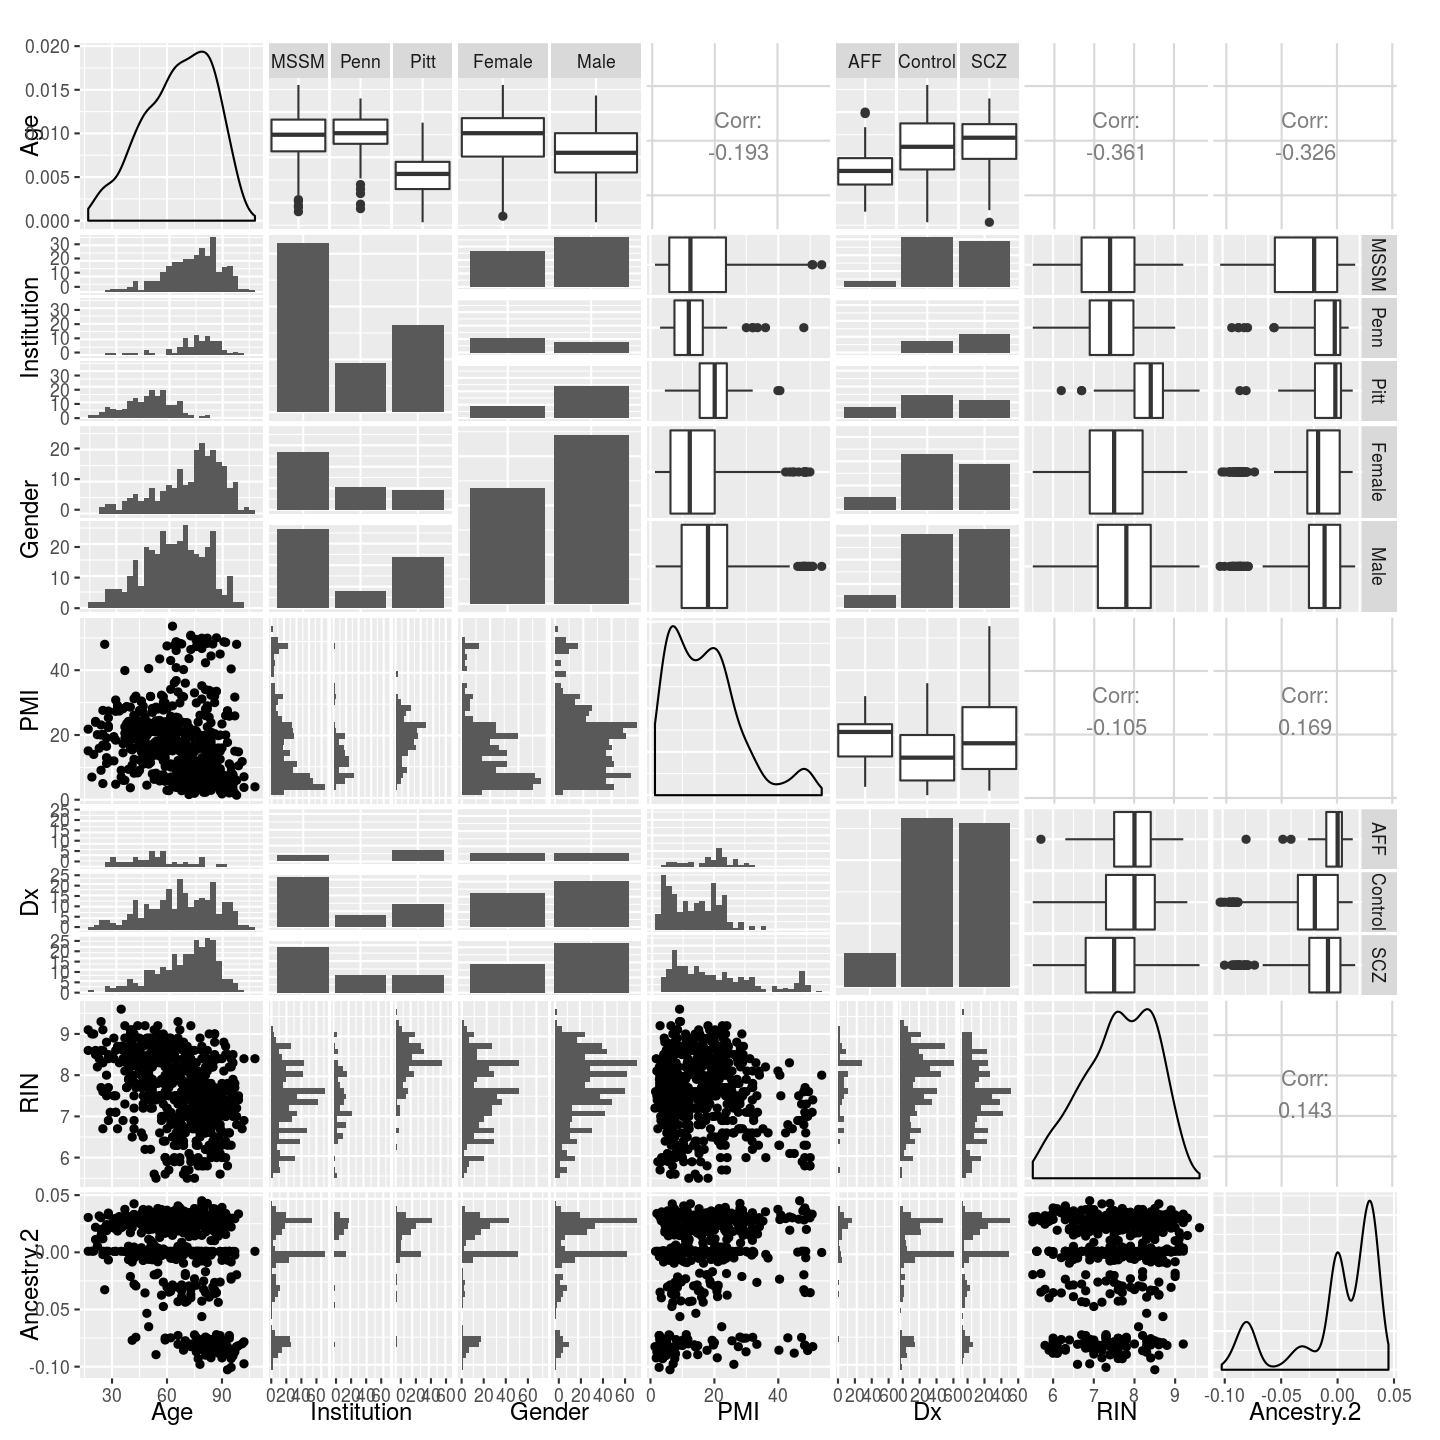
\includegraphics[scale=0.6]{figures/2016-06-26-trellis-display-of-data/evar-scatterplot-matrix-2.png}
\end{center}
\caption{
Distribution and inter-dependence of explanatory variables.  The diagonal graphs of the
plot-matrix show the marginal distribution of six variables (Age,
Institution,...)~while the off-diagonal graphs show pairwise joint
distributions.  For instance, the upper left graph shows that, in the whole
cohort, individuals' Age
ranges between ca.~15 and 105 years and most individuals around 75 years; the
bottom and right neighbor of this graph both show (albeit in different
representation) the joint distribution of Age and Institution, from which can
be seen that individuals from Pittsburg tended to be younger than those from
the two other institutions.
}
\label{fig:predictor-associations}
\end{figure}

\begin{figure}[H]
\begin{center}
\includegraphics{figures/by-me/monoall-dependencies-2/obs-simple-general/obs-simple-general}
\hspace{\fill}
\includegraphics{figures/by-me/monoall-dependencies-2/obs-simple-general-gene-aspec/obs-simple-general-gene-aspec}
\hspace{\fill}
\includegraphics{figures/by-me/monoall-dependencies-2/mixed/mixed}
\end{center}
\caption{ General dependency structures in two fixed effects regression models
(\emph{left}, \emph{middle}) and a mixed effects model (\emph{right}).  In all
three cases the regression coefficients \(\beta_{1g},...,\beta_{3g}\) or
\(\beta_{1g},b_{2g},b_{3g}\) mediate, for a given gene \(g\), probabilistic
dependencies (arrows) between the response variable \(Y_g\) (read count ratio
for \(g\)) and the corresponding explanatory variables \(X_1,...,X_3\).  For
simplicity but without loss of generality only 3 explanatory variables are
depicted.  The model frameworks differ in how the coefficients relate to each
other for a given explanatory variable (or a given \(j\)).  \emph{Left:} there
is no connection among \(\beta_{jg_1},\beta_{jg_2},...\) which means that the
way \(Y_{g}\), the read count ratio for gene \(g\) depends on variable \(X_j\)
is completely separate from how the read count ratio for any other gene \(g'\)
(i.e.~\(Y_{g'}\)) depends on it.  Consequently no information may be shared
among gene-specific models.  \emph{Middle:} In this case
\(\beta_{jg_1}=\beta_{jg_2}=...\equiv\beta_j\) so that all genes are identical
with respect to how their read count ratio depends the explanatory variables.
Thus genes share all information in the data in the sense that the model
forces them to be identical.  \emph{Right:} Hierarchical mixed effects model
where certain dependencies (\(\beta_1\)) are shared among genes while others
(\(\{b_{2g}\}_g, \{b_{3g}\}_g\)) vary across genes.  The variation is controlled by the
variance parameters \(\sigma^2_j\).  In this example there is a single set
\(\{b_{2g}\}_g\) of random coefficients for \(X_2\)---and a similar set for
\(X_3\)---, which are random intercepts.  In general, however, one or more set
of random slope coefficients may also be present.  Given the estimates
\(\hat{\sigma}^2_j\) and the data the gene-specific random coefficients
\(b_{jg}\) can be predicted.  Among the three only this model framework allows
information sharing among genes in a flexible way.  }
\label{fig:glm-vs-hierarch}
\end{figure}

\begin{figure}[H]
\begin{center}
\includegraphics[scale=0.6]{figures/2017-03-08-model-checking/qqplot-families-M3-1.pdf}
\end{center}
\caption{
Checking the fit of various model families: analysis of the normality of residuals.
}
\label{fig:qqnorm-mixed}
\end{figure}

\begin{figure}[H]
\begin{center}
\includegraphics[scale=0.6]{figures/2017-03-08-model-checking/scedasticity-families-M3-1.pdf}
\end{center}
\caption{
Checking the fit of various model families: analysis of homoscedasticity.
}
\label{fig:homoscedas-mixed}
\end{figure}

\begin{figure}[H]
\begin{center}
\includegraphics[scale=0.6]{figures/2017-07-31-mixed-model-coefs/ranef-gender-gender-gene-m5-all-panels-1.pdf}
\end{center}
\caption{
Predicted random coefficients \(b_{gj}\) for gene \(g\) (\(y\)-axis) and
random effect \(j\) (panel headers). Positive and negative coefficient indicates direct positive and
negative dependence of the given gene's read count ratio on age, respectively,
while zero coefficient suggests independence of age.  Compare with
Fig.~\ref{fig:S-age}.
}
\label{fig:pred-rnd-coefs}
\end{figure}

\clearpage

\subsection{Supplementary tables with legends}

\setcounter{table}{0}
\makeatletter 
\renewcommand{\thetable}{S\@arabic\c@table}
\makeatother

\begin{table}[H]
\begin{center}
\begin{tabular}{r|l}
explanatory variable & levels\\
\hline
Age &  \\
Institution & [MSSM], Penn, Pitt\\
Gender & [Female], Male\\
PMI & \\
Dx & [Control], SCZ, AFF \\
RIN &  \\
RNA\_batch & [A], B, C, D, E, F, G, H, 0\\
Ancestry.1 & \\
\vdots & \\
Ancestry.5 &  \\
\end{tabular}
\caption{ \emph{Left column:} explanatory variables of read count
ratio.  \emph{Right column:} levels of each factor-valued (i.e.~categorical)
variable.  Square brackets \([...]\) surround the baseline level against
which other levels are contrasted.  \emph{Abbreviations:} PMI: post-mortem
interval; Dx: disease status; AFF: affective spectrum disorder; SCZ:
schizophrenia; RIN: RNA integrity number;
Ancestry.\(k\): the \(k\)-th eigenvalue from the decomposition of genotypes
indicating population structure.}
\label{tab:predictors}
\end{center}
\end{table}

\begin{table}[H]
\begin{center}
\begin{tabular}{ccc}
%\multicolumn{2}{c}{\replaced{link function and error distribution}{regression models}} \\
model family & abbrev. & response var.~\\
\hline
\emph{u}nweighted \emph{n}ormal \emph{l}inear & unlm  & \(S, Q,\) or \(R\) \\
\emph{w}eighted \emph{n}ormal \emph{l}inear & wnlm  & \(S, Q,\) or \(R\) \\
\emph{logi}stic & logi & \(S\) \\
\emph{logi}stic, \(\frac{1}{2}\times\) down-scaled link fun.~& logi2 & \(S\) \\
\end{tabular}
\caption{Fitted regression model families, in which the response variable is the read count ratio with or without some transformation: 
\(S\)---untransformed, \(Q\)---\emph{q}uasi-log-transformed, and
\(R\)---\emph{r}ank-transformed read count ratio.  Diagnostic plots
(Fig.~\ref{fig:qqnorm-mixed},~\ref{fig:homoscedas-mixed}) and monitoring
convergence suggested that the \(\mathrm{unlm}.Q\) combination allows the
best fit for several linear predictors tested.
}
\label{tab:model-names}
\end{center}
\end{table}

\end{document}
